%!TEX root = ../master.tex
\section{Cryptography}\label{cryptography}
This section will briefly introduce concepts from cryptography relevant to the project, and will be based on \cite{cryptoenginering}.

\subsection{Encryption}
Encryption is a concept used for keeping the contents of messages between two parties secure.

When Alice sends a message to Bob over some insecure channel it is impossible to ensure that Eve does not read the message.
It is therefore safe to assume that a message sent by Alice to Bob can be read by Eve.
The situation can be seen on \cref{crypto:noenc}.

\begin{figure}[H]
	\centering
	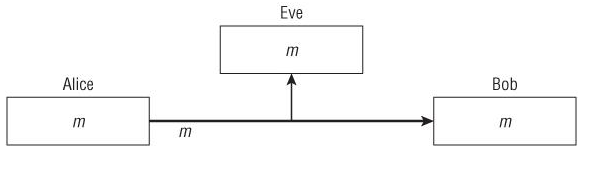
\includegraphics[width=0.6\textwidth]{encryptionNoEnc}
	\caption{Eve easily intercepts and reads \emph{m}.s From \citet[p.~50]{cryptoenginering}}
	\label{crypto:noenc}
\end{figure}

The solution is to encrypt the message \emph{m} with a key $K_e$ that is agreed on beforehand.
Now Alice can send an encryted message to Bob which Eve will be able to read but not understand.
The situation is presented on \cref{crypto:enc}.

\begin{figure}[H]
	\centering
	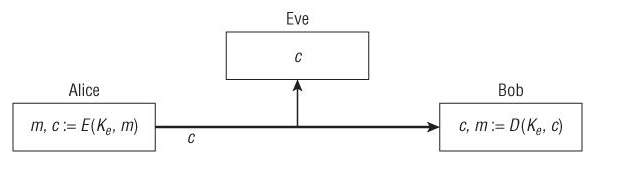
\includegraphics[width=0.6\textwidth]{encryptionSetup}
	\caption{Eve can still intercept but cannot understand \emph{m}. From \citet[p.~50]{cryptoenginering}}
	\label{crypto:enc}
\end{figure}

The encryption function is written as $c = E(K_e,m)$ where \emph{c} is the resulting cipthertext.
When Bob receives \emph{c} he can decrypt it with the encryption function written as $m = D(K_e,c)$.
Eve receives the same \emph{c} but does not have the encryption key and cannot read the original cleartext from it.
A good encryption further protects the cleartext even further by making it impossible for Eve to learn any information about \emph{m} besides the length and the time it was sent.


\subsection{Authentication}
Authentication is a concept used for ensuring that the traffic between two parties are being tampered with.

When Alice sends messages to Bob over some insecure channel it can be possible for Eve to change how Bob receives the messages.
Eve can alter the sent message \emph{m} to \emph{m'} and send \emph{m'} to Bob without Bob knowing.
Eve can also change the order of messages so a message comes much later than intended.
If Eve deletes a message Bob will never know that this message existed.
Eve can even create her own message and send it without Bob can know that this message was not created by Alice.

\begin{figure}[H]
	\centering
	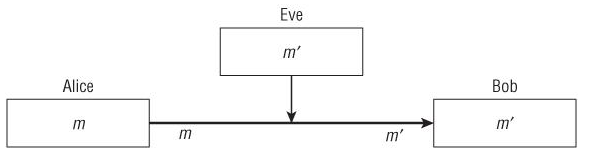
\includegraphics[width=0.6\textwidth]{authenticationNoAuth}
	\caption{The basic problem, who sent \emph{m'}? From \citet[p.~52]{cryptoenginering}}
	\label{crypto:noauth}
\end{figure}

Part of the solution to these problems is authentication of messages \citet[p.~52]{cryptoenginering}.
Alice and Bob have a shared secret key $K_a$ for authentication.
When sending message \emph{m} Alice first computes a Message Authentication Code (MAC).
This authentication code \emph{a} is calculated as $a := h(K_a,m)$, where $h()$ is the MAC function.
Alice now sends both the MAC \emph{a} and the message \emph{m} to Bob.
When Bob receives \emph{a} and \emph{m} he computes the MAC of \emph{m} and compares with the \emph{a} he received from Alice.
The situation is outlined on \cref{crypto:authsetup}

\begin{figure}[H]
	\centering
	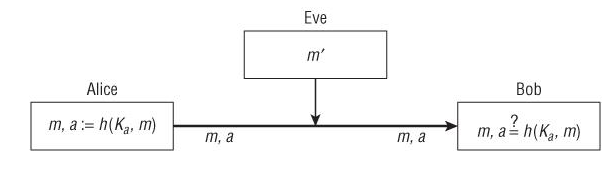
\includegraphics[width=0.6\textwidth]{authenticationSetup}
	\caption{Setup for authentication. From \citet[p.~53]{cryptoenginering}}
	\label{crypto:authsetup}
\end{figure}

If Eve wants to modify the message \emph{m} to the different message \emph{m'} and simply replaces \emph{m} with \emph{m'}, Bob will be able to tell when computing the MAC of \emph{m'}.
This is the case because of the design of the MAC function.
A MAC function is designed such that two different messages \emph{m} and \emph{m'} are very unlikely to result in the same MAC.
Bob will therefore discard message \emph{m} as an attacked message.

Even with this countermeasure Eve will be able to record a message and MAC pair and send it to Bob at a later point in time.
She can also still delete messages without Bob knowing that it ever existed.
Because of these flaws authentication is almost always accompanied by a numbering scheme which makes it possible for Bob to determine if there is being tampered with the message order.
Eve will still be able to entirely stop the communication between Alice and Bob, or delay it.
